The Google Android operating system was chosen as the client platform. This
decision was based primarily on two factors, firstly that the teams mobile
development experience was mainly with Android and additionally the
availability of development hardware for the duration of the project.

As a part of our white-boarding meetings, we developed a high level idea of the
functionality required by the client interface this can be seen in
Figure~\ref{fig:system_components}.

To create a structure for the client the team explored a number of low fidelity
user interface options. The agreed upon interface was used as a basis to create
an architecture for the project. The identified components and their
communications are described in Figure~\ref{fig:client_design}.

\begin{figure}[htb]
\centering
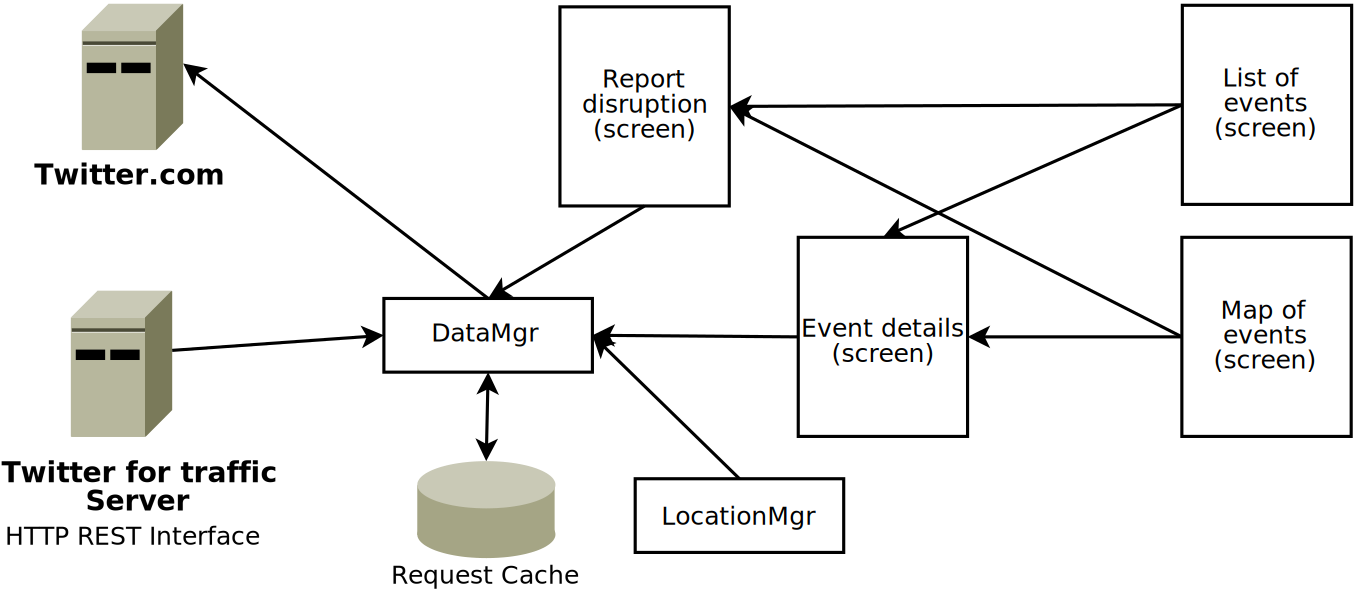
\includegraphics[width=0.9\textwidth]{images/design/client/client_high_level_layout.pdf}
\caption{High level client design}
\label{fig:client_design}
\end{figure}


\subsubsection{Server interface}
As previously discussed in this document, a ‘mock’ server was created to
parallelise efforts and to verify the REST endpoints. This tool proved very
useful in the development of the client application, particularly with verbose
logging on the server side when debugging connection issues.

The interaction with the server is encapsulated in the \emph{DataMgr} class.
This class returns lists of the relevant object types to the requester. The
interface for this class can be seen in Listing \ref{datamgrinterface}.

\lstset{caption={DataMgr.class public interface},label=datamgrinterface}

\begin{lstlisting}
public DataMgr(Context context);
public List<EventItem> requestEvents();
public List<TweetItem> requestTweets(String eventID);
public List<EventItem> requestRouteEvents(Route route);
\end{lstlisting}

\subsubsection{Request caching}
Modern mobile data networks have increased data-rates to an incredible level
over the last number of years, it is not uncommon now to see providers offering
speeds of 7.2 Mbps. But these types of networks also tend to incur large
latencies, for an initial TCP request from mobile handset round trip times of
up to one second are not unheard of.

As a mechanism to make the application feel more responsive to the user, the
application caches the response from the previous request. This cached response
is displayed if delays or issues occur but once fresh data becomes available
the screen is populated with this data. Most typically delays occur in
acquiring a geographical lock, as we require a current geographical location to
make an event request. Or being unable to contact the server due to
connectivity issues.

\subsubsection{Twitter interface}
\subsubsection{Home route functionality}
\subsubsection{User interface}
